%%%% NQM %%%%
\section{NCA Quality Metric (NQM)}
\label{methods:NQM}
\begin{figure}
    \centering
    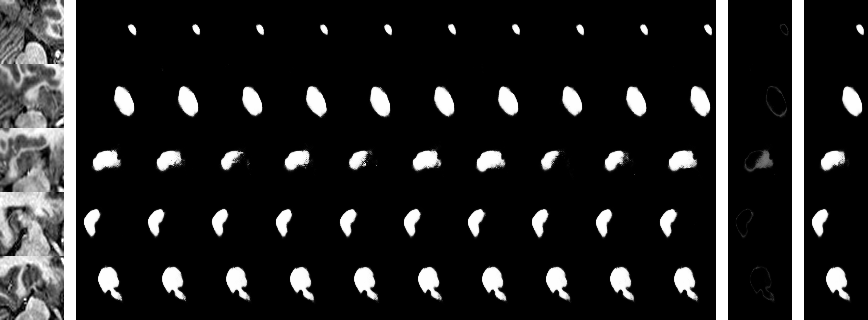
\includegraphics[width=\linewidth]{Graphics/nqm_stack10_epoch_50_var_mu.png}%{Graphics/nca_random_outputs.png}
    \caption{From left to right: Inputs, 10 predictions, Variance, and Mean. As seen here, NCAs produce different outputs on identical inputs each time they are called. Each of the 10 predictions here are outputs of the same model. Therefore, as shown on the right, one can compute a variance and a mean over these predictions. The NQM we introduce here for model optimization reduces this to single values. The outputs are generated from a model in an earlier training state for better visualization.}
    \label{fig:nca_random_outputs}
\end{figure}

%%%% random activation + image example %%%%
As seen in \autoref{methods:NCA}, NCAs are activated randomly to a certain extent. Therefore, they generate different predictions each time they are called, especially with the same input. Examples can be seen in \autoref{fig:nca_random_outputs}. On the far left, one can see five different inputs. Next to them are ten outputs from the same model, shown here for better visualization at an early stage of training. Especially for the middle input, the differences in the outputs can be seen quite well with the naked eye. For the other inputs, the variance over these ten outputs (the second last column on the right) also clearly shows that the model produces different outputs for all input images. Otherwise, the variance should be zero, i.e., completely black. The variance decreases for models with higher epochs but never disappears. It also remains the case that the variance for some inputs is significantly worse than for others.

%%%% Def NQM, from/like John %%%%
\autocite{kalkhof:2023:M3D-NCA} introduced a way to measure this stochasticity of NCAs, caused by random activation, by computing a mean-normalized variance over a stack of such generated outputs and named it the NCA-\textit{Quality-Metric} (NQM). \autocite{kalkhof:2023:M3D-NCA} used this to detect bad segmentation on artificially degenerated data automatically. They defined it as follows, with $v$ as the image volume and $v_i$ as $N=10$ different predictions:

\begin{align}
    \mathrm{NQM} := \frac{\sum_{s\in SD} (s)}  {\sum_{m\in\mu}}, \qquad
    \mathrm{SD} = \sqrt{\frac{\sum^N_{i=1}(v_i-\mu)^2}  {N}}, \qquad
    \mu = \frac{\sum^N_{i=1}v_i}  {N}
\end{align}


This approach has given rise to the question of whether it is possible somehow to pull the NQM inside the training circle, to improve the robustness of the models and not just for the final evaluation. What has been addressed with this thesis. 


%%%% Why to put NQM in the Loss %%%%
The NQM is a single scalar value greater than or equal to zero. With the NQM, a model will perform better if the NQM is smaller. Therefore, the goal of optimizing a model with respect to the NQM can be formalized as a direct minimization problem over the NQM $\min(\text{NQM})$. Other approaches are possible, as discussed in \autoref{conclusions}. Since the object to optimize the NQM can be formalized as a minimization problem, and in the training cycle of a Neural Network, there is already an object to minimize, i.e., the loss, and NCAs are Neural Networks, it is very close to trying to minimize the NQM by using it as the loss function or by including the NQM in the loss function. This is also our approach in this work, and, as we will show, it can lead to a more robust behavior of the model. I.e., it can improve the robustness of the model, as we will see in \autoref{experiments:intro} especially in \autoref{experiments:03.1.0:backbone_hippo:intro}. In \autoref{experiments:03.2.0:med_prost:intro}, \ref{experiments:03.3.0:med_hippo:intro_and_Augmented}, and \ref{experiments:03.4.0:backbone_prost:intro}, we will also see that this is not trivial to transfer to other models and datasets, and that some models may even become less robust.


%%%% Schlussanmerkung  -> evt. nach Conclusions %%%%
The NQM, and therefore this approach, is limited to NCAs and possibly other models with randomness in the output since it is a metric over that randomness. Therefore, the NQM and everything related to it in this paper does not work for most other Neural Networks since the output with these is deterministic.